% --------------------------------------------------------------------------- %
\chapter{Программная реализация}\label{chap3_soft_architecture}
% --------------------------------------------------------------------------- %
\section{Архитектура}
% --------------------------------------------------------------------------- %
\subsection{Описание элемента состояния данных}
Текущая реализация ``графоориентированного подхода'' в библиотеке comsdk поддерживает обработку данных следующих типов:
\begin{itemize}
    \item целые числа,
    \item числа с плавающей точкой,
    \item строки,
    \item числовые векторы,
    \item ассоциативные массивы с строковыми ключами.
\end{itemize}

Для их представления в разрабатываемой библиотеке был объявлен перечислимый тип \textsf{DType} (рис.~\ref{fig:UMLDatatype}).

\begin{figure}
    \centering
    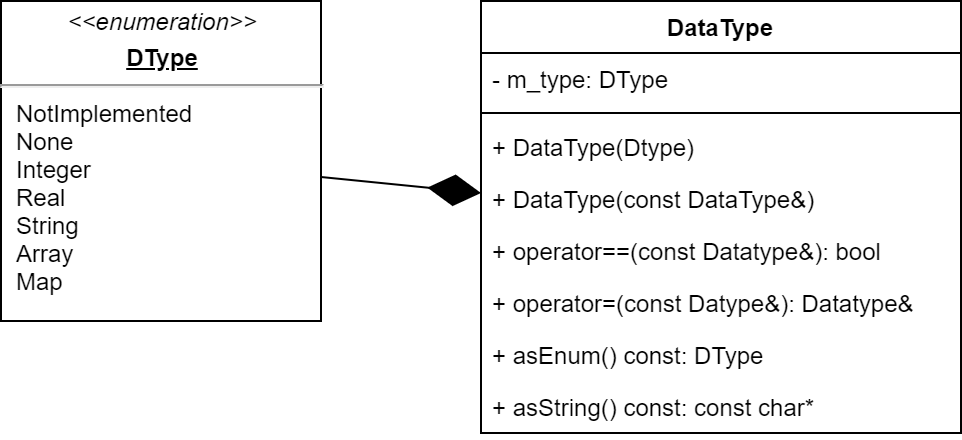
\includegraphics[width=0.6\textwidth]{figures/UML.datatype.png}
    \caption{UML-диаграмма структуры данных для описания типов используемых данных}
    \label{fig:UMLDatatype}
\end{figure}

Помимо перечисленных выше типов присутствуют два дополнительных: None и NotImplemented. Данные типы используются для обозначения ошибок и исключительных ситуаций.

Класс \textsf{DataType}, представленный на рисунке~\ref{fig:UMLDatatype} хранит только числовую константу, обозначающую тип и реализует некоторую дополнительную функциональность, а именно:
\begin{itemize}
    \item даёт возможность присываивать и сравнивать типы при помощи соответсвующих перегруженных операторов;
    \item даёт возможность получить имя типа при помощи метода \textsf{asString()}.
\end{itemize}

Для каждого из поддерживаемых на данный момент типов данных был создан константый объект класса DataType, содержащий в себе описание этого типа. Константы имеют следующие имена: \textsf{dInt}, \textsf{dReal}, \textsf{dString}, \textsf{dVector}, \textsf{dMap}. Кроме того, были объявлены две дополнительные константы для описания ситуации, когда запрашиваемый элемент не найден -- \textsf{dNone} -- и для ситуации, когда у запрошенной операции отсутствует реализация -- \textsf{dNotImplemented}.

На рисунке~\ref{fig:UMLElement} представлена UML-диаграмма основного класса, описывающего элемент состояния данных.

\begin{figure}[!ht]
    \centering
    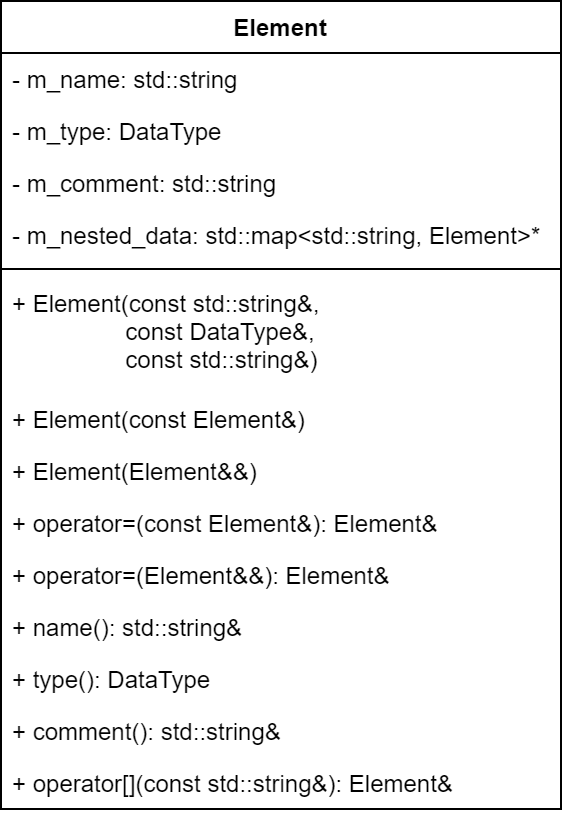
\includegraphics[height=0.33\textheight]{figures/UML.element.png}
    \caption{UML-диаграмма структуры данных для описания элемента состояния данных}
    \label{fig:UMLElement}
\end{figure}

В классе \textsf{Element} поля \textsf{m_name}, \textsf{m_type} и \textsf{m_comment} хранят в себе имя элемента, его тип (целочисленный, с плавающей точкой, строковый, числовой векторный, ассоциативный массив) и краткое описание соответственно. Закрытое поле \textsf{m_nested_data} содержит указатель на ассоциативный массив объектов типа Element. Данное поле используется, если сам элемент имеет тип ассоциативного массива (\textsf{dMap}). Поскольку элементы такого массива могут иметь разные типы, целесообразно для каждого такого элемента хранить их ключи и типы. Таким образом, каждый элемент ассоциативного массива по своей структуре повторяет элемент состояния данных. Это свойство позволяет делать состояния данных иерархическими. Использование указателя на объект std::map позволяет эффективнее использовать память в случае, когда тип элемента отличен от ассоциативного массива и нет необходимости обеспечивать доступ к его внутренним элементам.

Конструктор класса принимает на вход две строки и объект класса DataType, которые соотносятся с полями \textsf{m_name}, \textsf{m_comment} и \textsf{m_type} соответственно. Были явно реализованы конструктор копирования и оператор присваивания, поскольку в классе используются указатели на память, за выделение и освобождение которой отвечает он сам.

Для работы с элементами ассоциативного массива был реализован метод доступа по ключу (\textsf{operator[]}). При отсутствии элемента с запрошенным ключом в массиве он должен создаваться. Во избежание неопределённого поведения (англ. undefined behaviour) при вызове данного метода у элемента, тип которого отличен от ассоциативного массива (\textsf{Map}), метод будет возвращать специальную константу NotImplemented с одноимённым типом и пустым именем. Кроме того, для const-версии этого метода была добавлена проверка на наличие элемента в массиве. В случае его отсутствия будет возвращена константа None, имеющая одноимённый тип и пустую строку в качестве имени.

% --------------------------------------------------------------------------- %
\subsection{Описание состояния данных}
% --------------------------------------------------------------------------- %

На рисунке~\ref{fig:UMLDatastate} представлена UML-диаграмма разработанного класса, отвечающего за представление всего состояния данных вычислительного метода.

\begin{figure}[!ht]
    \centering
    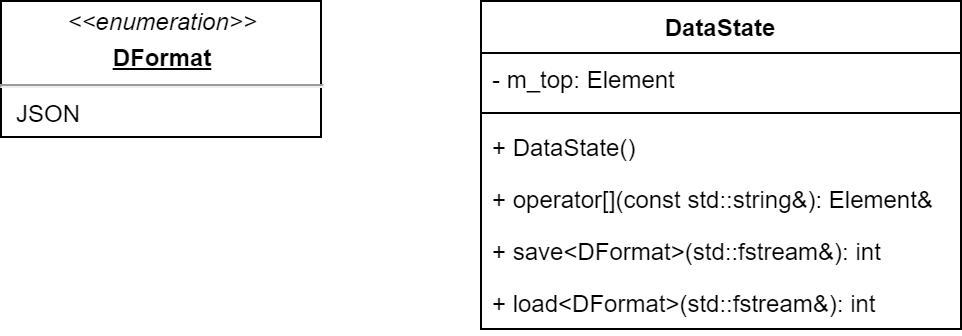
\includegraphics[width=0.6\textwidth]{figures/UML.datastate.png}
    \caption{UML-диаграмма класса, представляющего состояние данных}
    \label{fig:UMLDatastate}
\end{figure}

Единственным закрытым членом этого класса является объект класа \textsf{Element}, который является ``корневым'' элементом состояния данных. Он имеет имя ``root'' и всегда имеет тип \textsf{Map}, и все элементы самого состояния данных хранятся внутри корневого элемента. При этом их ключи совпадают с их именами. Это даёт интуитивный интерфейс для взаимодействия с иерархической структурой состояния данных.

В классе \textsf{DataState} объявлены два шаблона метода загрузки состояния данных из файла и его сохранения в файл. Параметром шаблона является переменная перечислимого типа \textsf{DFormat}, в котором определены возможные файловые форматы, с которыми возможно взаимодействие. Подобный подход позволяет создавать различные реализации загрузки и сохранения состояний данных с сохранением единого интерфейса, что положительным образом сказывается на расширяемости разработанной кодовой базы.

% --------------------------------------------------------------------------- %
Общая структура разработанных классов представлена на рисунке~\ref{fig:UMLAll}
\begin{figure}[!ht]
    \centering
    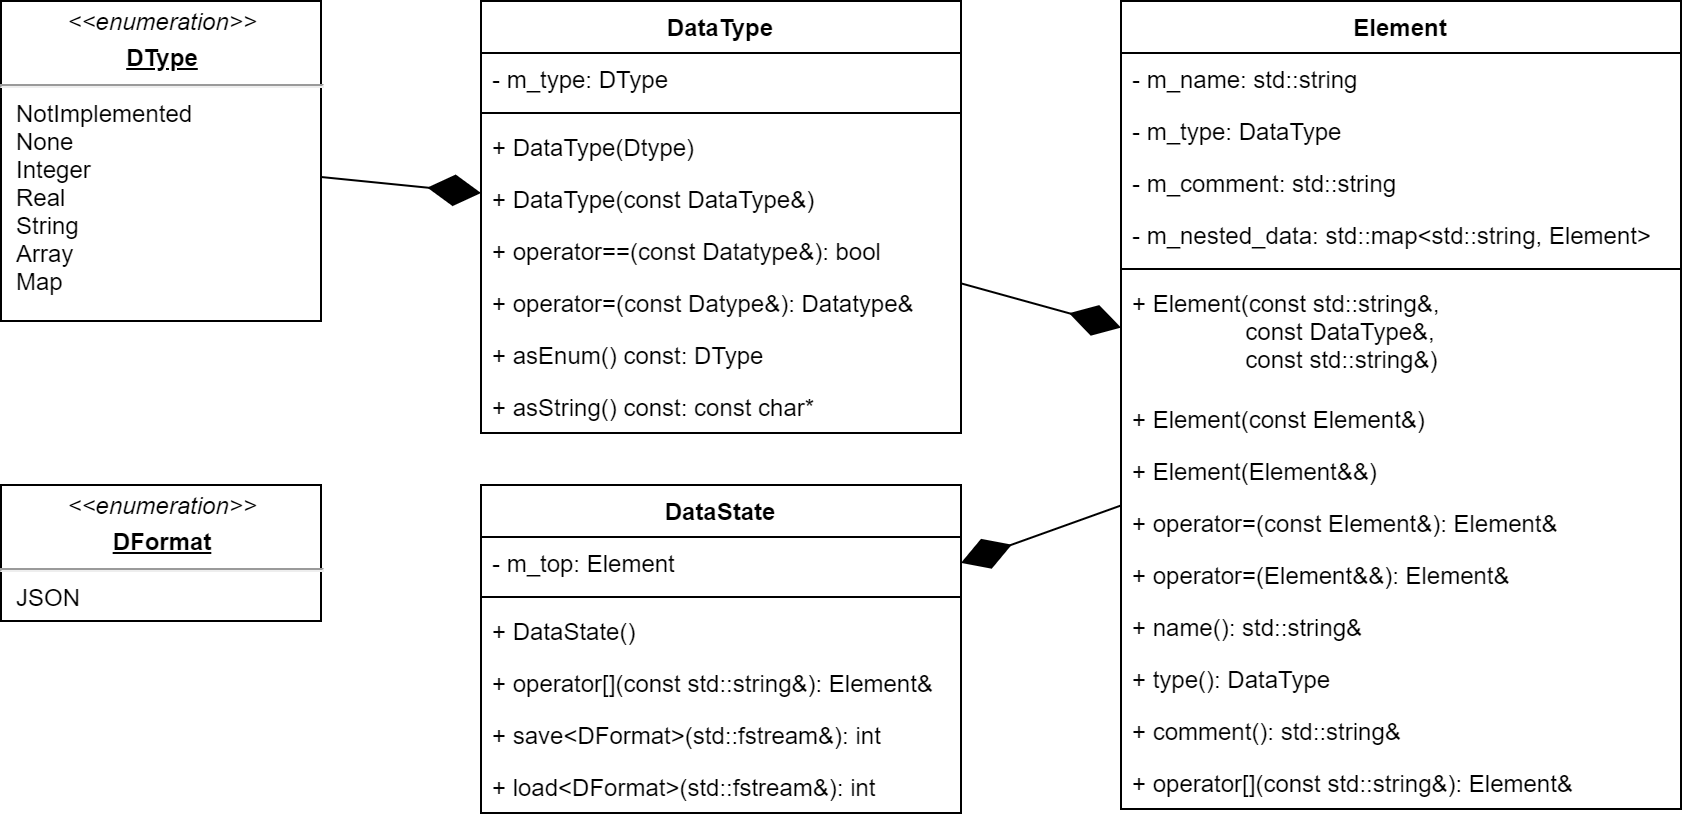
\includegraphics[width=0.9\textwidth]{figures/UML.all.png}
    \caption{Структура разработанных классов}
    \label{fig:UMLAll}
\end{figure}

%----------------------------------------------------------

